\chapter{具体设计样例}\label{chap:design}

\section{抑郁症模型的需求}\label{sec:depression-model-requirement}
抑郁症是一种复杂的神经系统疾病,涉及神经和生化过程的多种紊乱。
尽管已有大量研究致力于抑郁症的机制研究,但现有的动物模型仍存在诸多争议。
脑类器官为抑郁症的研究提供了一个新的实验平台,能够更好地模拟人类大脑的功能和病理变化。

\begin{figure}[!htbp]
    \centering
    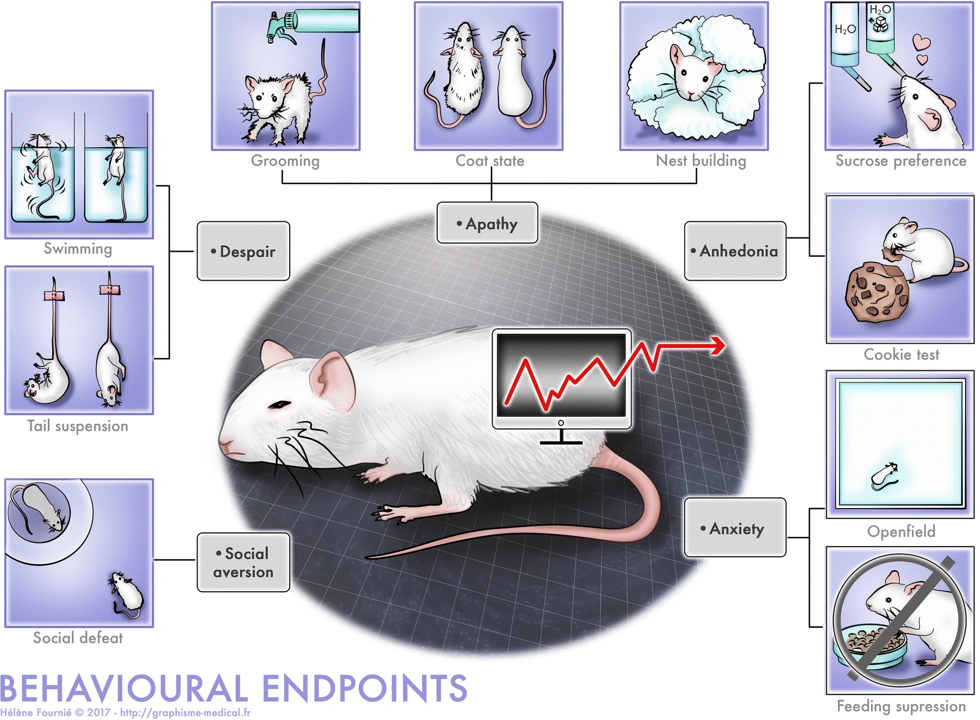
\includegraphics[width=0.75\textwidth]{Img/depression-model.png}
    \bicaption{现有的抑郁症动物模型示意图}{Existing Animal Models of Depression}
    \label{fig:depression-model}
\end{figure}

\section{研究目标}\label{sec:research-objective}
本研究的目标是通过结合电刺激和化学刺激,训练出一个功能性的健康海马体脑类器官。
在此基础上,引入常见的抑郁症诱导机制,如毒性化合物和电刺激,诱导海马体脑类器官进入疾病状态。
这一研究将为抑郁症的机制研究和药物筛选提供新的实验模型。


\section{实验设计}\label{sec:experiment-design}
\subsection{宏观培养}\label{subsec:macro-culture}
首先,将 hiPSC 分化为海马体神经元\cite{Wu2024},并直接在微电极阵列(MEA)芯片上进行培养。
通过精确控制培养条件,确保海马体脑类器官的形态和功能与真实大脑相似。

\begin{figure}[!htbp]
    \centering
    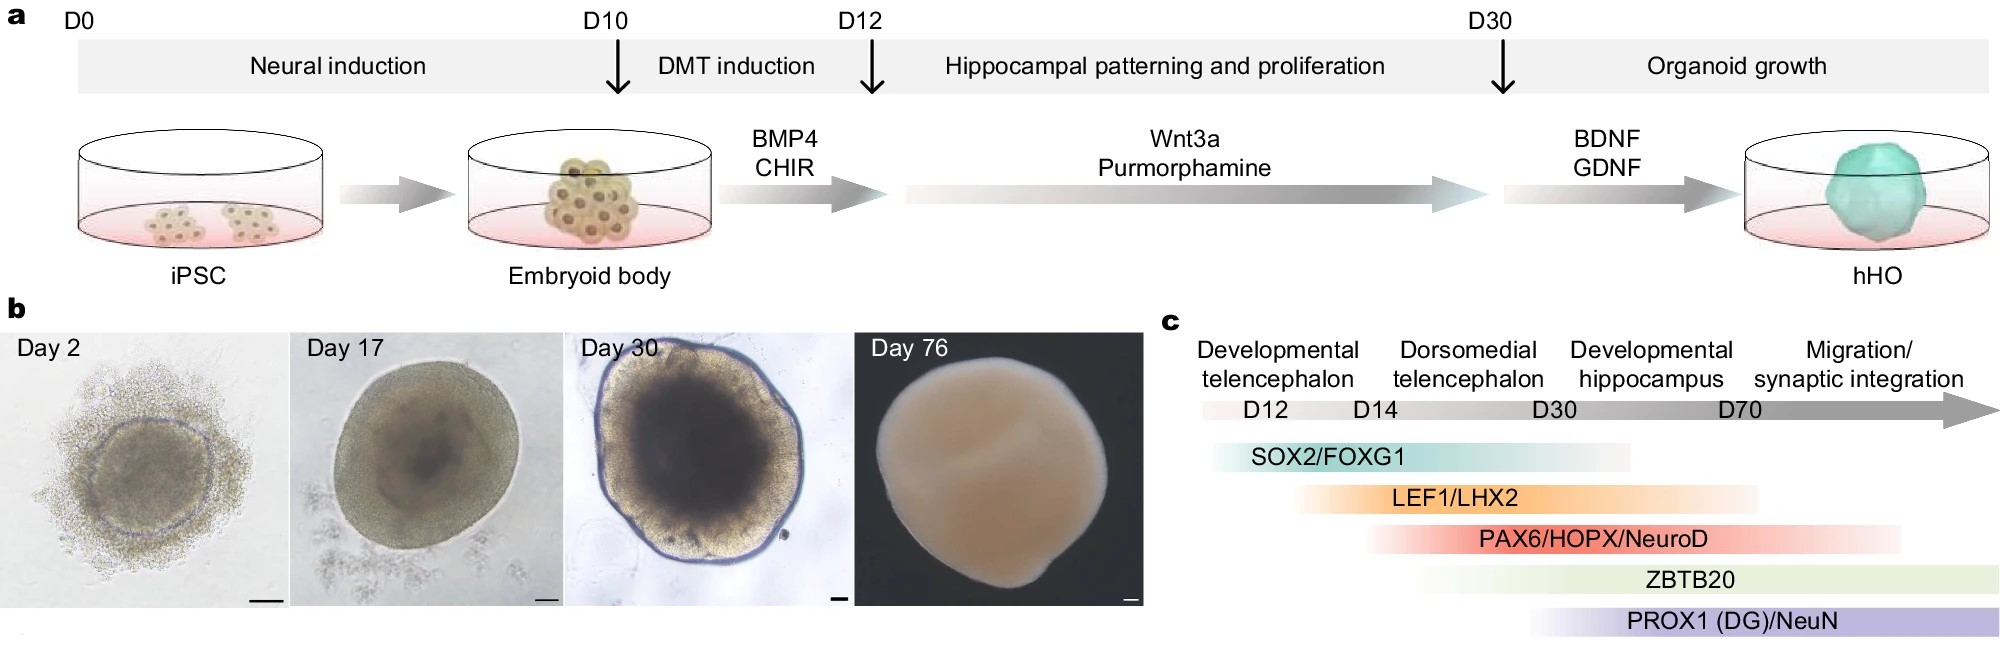
\includegraphics[width=0.75\textwidth]{Img/hipp-organoid.jpg}
    \bicaption{海马体脑类器官的培养示意图\cite{Wu2024}}{Schematic Diagram of Hippocampal Organoid}
    \label{fig:hipp-organoid}
\end{figure}

\subsection{微观培养}\label{subsec:micro-culture}
在微观培养阶段,通过外部刺激作为奖励或惩罚信号,训练海马体脑类器官的神经网络。
这一过程将帮助脑类器官形成功能性的神经网络,并模拟真实大脑的学习过程。

\begin{figure}[!htbp]
    \centering
    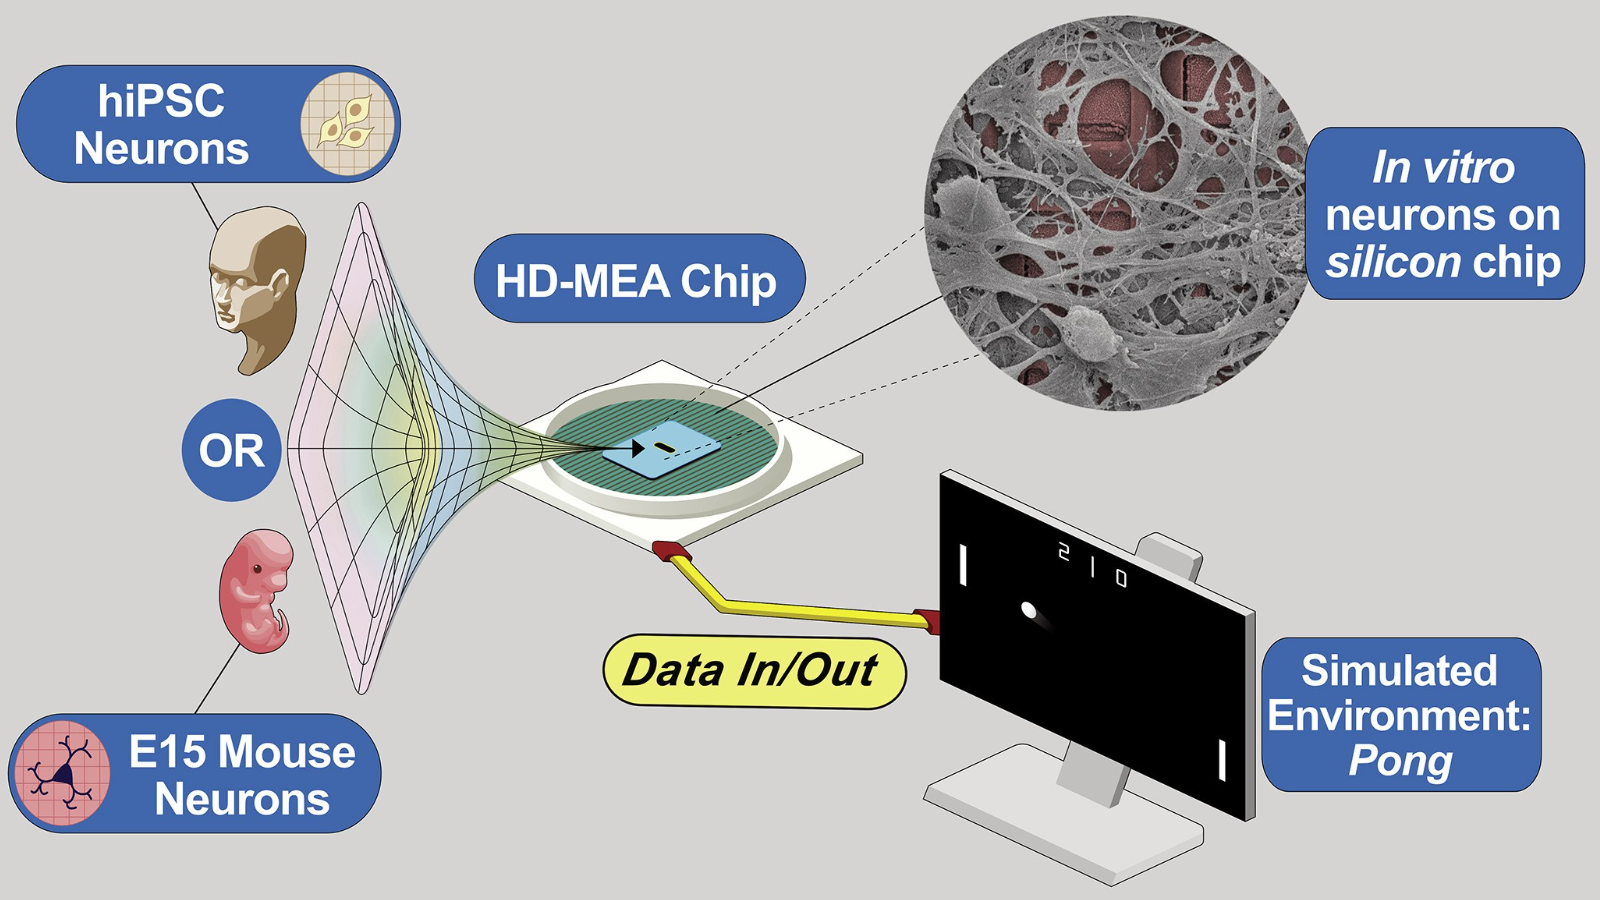
\includegraphics[width=0.75\textwidth]{Img/demo-dishbarin.png}
    \bicaption{盘中之脑的训练设计\cite{Kagan2022}}{Training Design of Dish Brain}
    \label{fig:demo-dishbarin}
\end{figure}

\subsection{抑郁症诱导}\label{subsec:depression-induction}
在脑类器官形成功能性神经网络后,引入抑郁症诱导机制。
通过使用皮质酮、IL-6 和 TNF-α 等化学物质,以及电刺激,诱导海马体脑类器官进入疾病状态。
这一过程将模拟抑郁症的病理变化,为研究抑郁症的机制提供新的实验平台。


\section{应用前景}\label{sec:application-prospect}
本研究提出的抑郁症模型具有广泛的应用前景。
首先,它为抑郁症的机制研究提供了一个创新的实验平台。
其次,该模型可以用于药物筛选,帮助开发新的抗抑郁药物。
最后,通过研究脑类器官在疾病状态下的网络水平变化,可以为理解精神健康障碍提供新的见解。


